\chapter{Metodologi dan Desain Sistem}

\section{Eksplorasi Data}
Eksplorasi data (\textit{Exploratory Data Analysis} / EDA) pada penelitian ini dilakukan untuk memahami karakteristik, distribusi, dan kualitas visual dari citra kerusakan jalan. Melalui analisis statistik dan visualisasi, EDA berperan penting dalam mengidentifikasi ketidakseimbangan kelas (\textit{class imbalance}) dan variasi ukuran objek untuk menentukan strategi pra-pemrosesan data yang tepat.

\subsection{Akuisisi Dataset}
Penelitian ini menggunakan dua jenis dataset yang diperoleh melalui metode akuisisi yang berbeda untuk memenuhi skenario pelatihan dan pengujian \textit{zero-shot}:
\begin{enumerate}
	\item \textbf{Data Sekunder (Dataset Pelatihan):} Dataset global \textcolor{blue}{\href{https://data.mendeley.com/datasets/27c8pwsd6v/3}{N-RDD2024}} yang merupakan perluasan dari RDD2022. Dari dataset ini, diekstraksi subset spesifik dari negara Asia (India, China, dan Jepang) dengan total 10.395 citra. Data ini sudah memiliki anotasi \textit{bounding box} untuk kelas kerusakan utama (D00, D10, D20, D40) serta kelas pengecoh (D70 untuk penutup saluran air dan D80 untuk tambalan jalan).
	\item \textbf{Data Primer (Dataset Pengujian \textit{Zero-Shot}):} Data citra jalan raya primer diakuisisi secara mandiri di wilayah Bandung. Pengambilan data difokuskan pada rute jalan raya dan jalan besar beraspal untuk merepresentasikan karakteristik infrastruktur lalu lintas utama di Indonesia. Target kuantitas data yang akan diekstraksi dan dianotasi adalah minimal 500 citra berlabel. Akuisisi dilakukan menggunakan kamera perekaman 1080p pada 30 fps dengan sudut pandang pengendara kendaraan roda dua pada kondisi siang hari. Frame diekstraksi dengan interval tertentu, misalnya setiap 1–2 detik atau berdasarkan perubahan \textit{scene}, untuk mengurangi redundansi visual antar citra. Karena data ini bersifat mentah, dilakukan pelabelan secara manual menggunakan perangkat lunak \textit{Computer Vision Annotation Tool} (CVAT) / Roboflow dengan format anotasi standar YOLO. Kualitas anotasi divalidasi secara manual untuk memastikan konsistensi label. Standar penarikan kotak pembatas (\textit{bounding box}) untuk seluruh kelas mengacu pada panduan contoh visual dari dataset N-RDD2024 beserta literatur basisnya, yakni RDD2022 \cite{Arya2024846}.

\end{enumerate}

\subsection{Visualisasi Data}
Tahap eksplorasi dan visualisasi data pada penelitian ini difokuskan pada subset data latih (\textit{training set}) N-RDD2024 dari tiga negara Asia: Jepang, Tiongkok, dan India. Mengingat dataset N-RDD2024 awalnya dikembangkan untuk keperluan kompetisi dengan label \textit{ground truth} pada data uji (\textit{test set}) yang dirahasiakan, maka seluruh proses eksplorasi ini hanya menggunakan data latih publik.

Dari total 10.395 citra awal, dilakukan proses penyaringan (\textit{filtering}) untuk mengekstraksi citra yang hanya memuat setidaknya satu dari enam kelas target penelitian (retakan memanjang, retakan melintang, retakan buaya, lubang jalan, penutup saluran, dan jalan bertambal). Proses penyaringan ini menghasilkan 9.670 citra siap pakai yang secara asli telah tersedia dalam format resolusi $640\times640$ piksel. Proporsi distribusi citra berdasarkan negara ditunjukkan pada Gambar \ref{fig:distribusi_negara}.

% ==========================================
% GAMBAR: DISTRIBUSI CITRA PER NEGARA
% ==========================================
\begin{figure}[H]
	\centering
	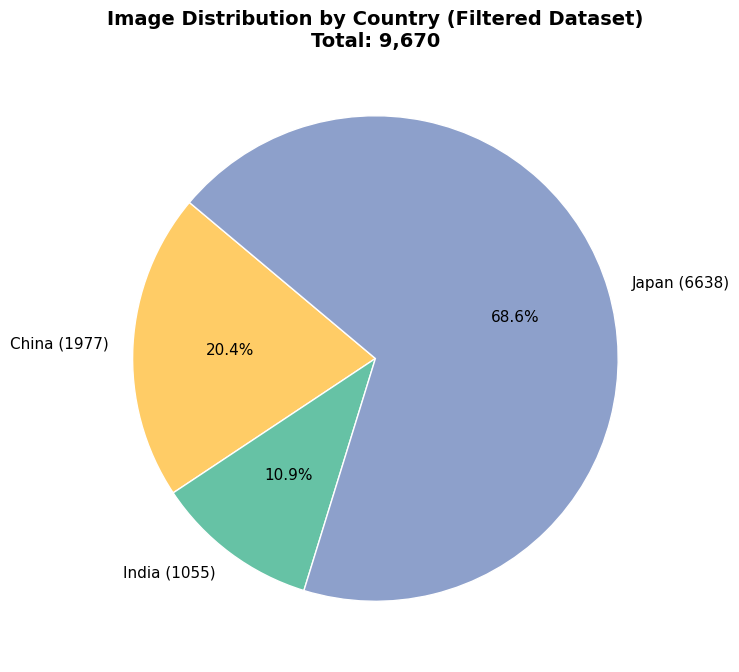
\includegraphics[width=0.7\textwidth]{gambar/distribusi_gambar.png} % Sesuaikan nama file
	\caption{Distribusi Citra N-RDD2024 Berdasarkan Negara}
	\label{fig:distribusi_negara}
\end{figure}

Berdasarkan Gambar \ref{fig:distribusi_negara}, terlihat bahwa dataset didominasi oleh citra dari Jepang sebanyak 6.638 citra (68,6\%), disusul oleh Tiongkok dengan 1.977 citra (20,4\%), dan India dengan 1.055 citra (10,9\%). Keragaman asal citra ini memunculkan variasi visual yang tinggi pada karakteristik jalan, sebagaimana divisualisasikan pada contoh citra anotasi kelas dan contoh perwakilan tiap negara di Gambar \ref{fig:contoh_kelas} dan Gambar \ref{fig:contoh_negara}.

% ==========================================
% GAMBAR: CONTOH KELAS
% ==========================================
\begin{figure}[H]
	\centering
	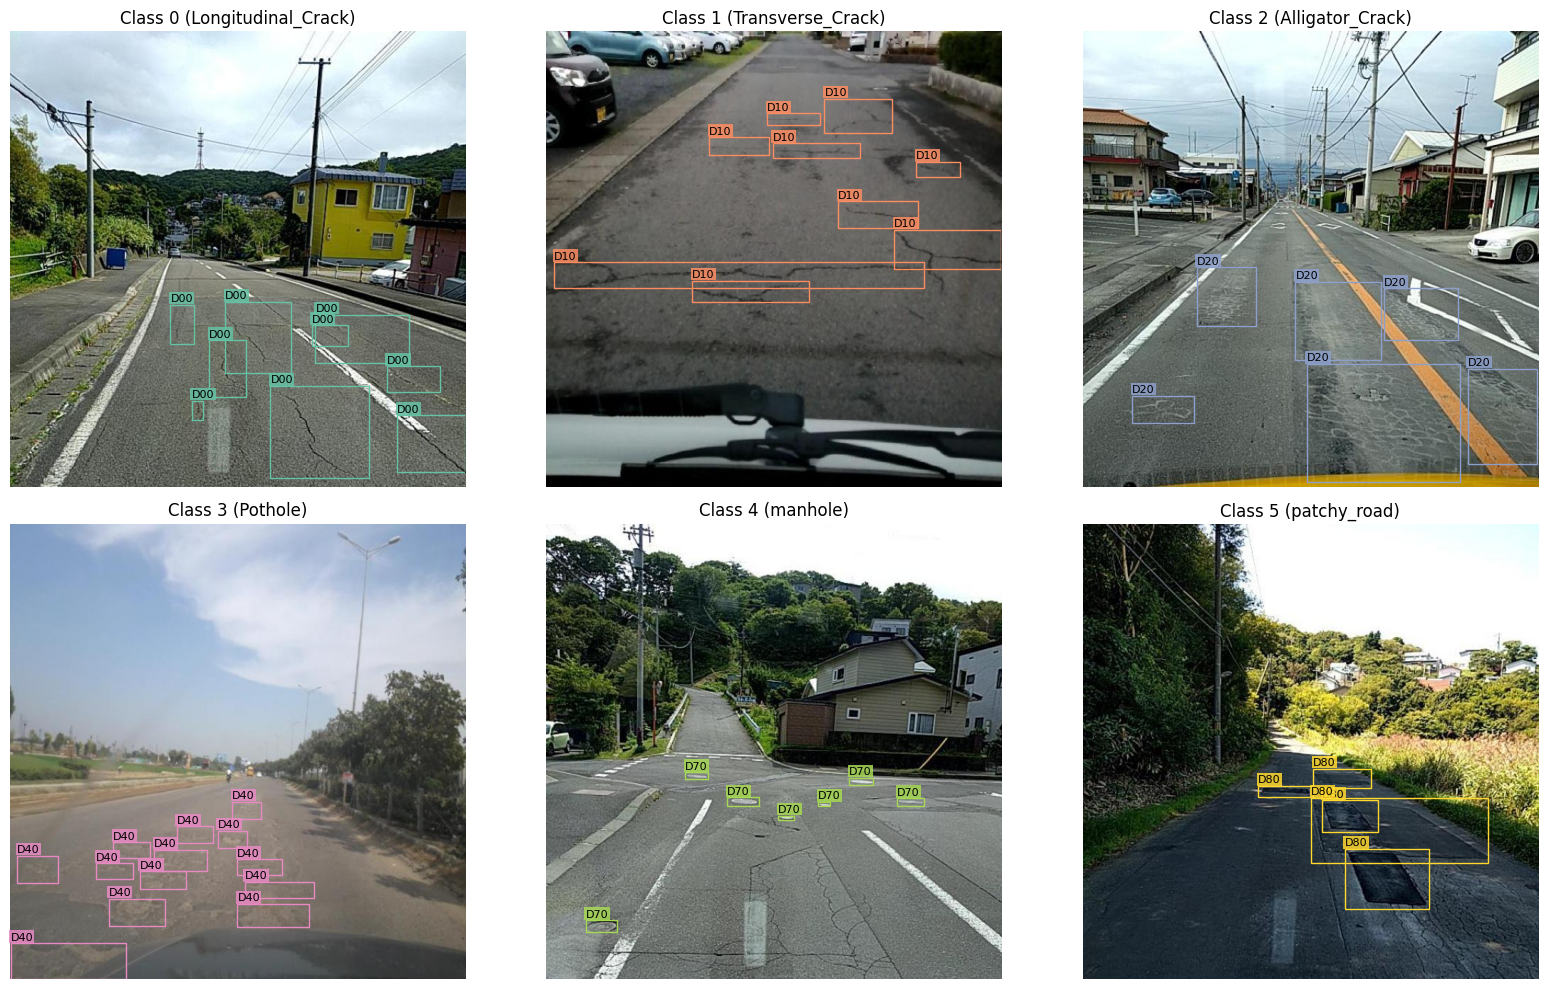
\includegraphics[width=0.9\textwidth]{gambar/object_sample.png} % Sesuaikan nama file
	\caption{Contoh Visualisasi \textit{Bounding Box} untuk Enam Kelas Target}
	\label{fig:contoh_kelas}
\end{figure}

% ==========================================
% GAMBAR: CONTOH NEGARA
% ==========================================
\begin{figure}[H]
	\centering
	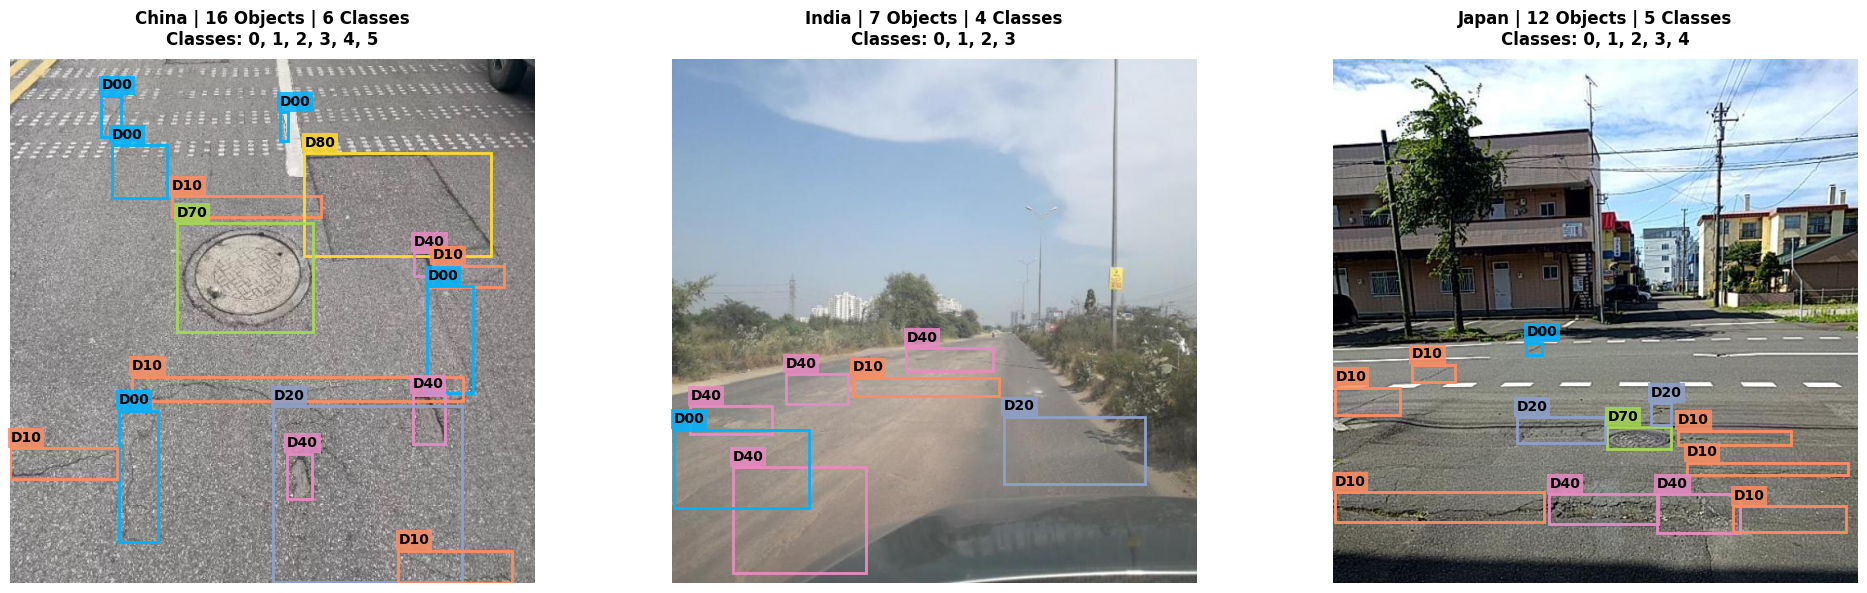
\includegraphics[width=0.9\textwidth]{gambar/object_per_country.png} % Sesuaikan nama file
	\caption{Contoh Perbedaan Karakteristik Citra Jalan di tiap Negara}
	\label{fig:contoh_negara}
\end{figure}

Selain asal negara, tantangan utama dari dataset ini terletak pada ketimpangan distribusi jumlah objek antar kelas (\textit{class imbalance}). Analisis terhadap total 24.290 objek berlabel menunjukkan bahwa kelas retakan struktural sangat mendominasi dibandingkan kelas anomali permukaan lainnya.

% ==========================================
% GAMBAR: DISTRIBUSI KELAS GLOBAL
% ==========================================
\begin{figure}[H]
	\centering
	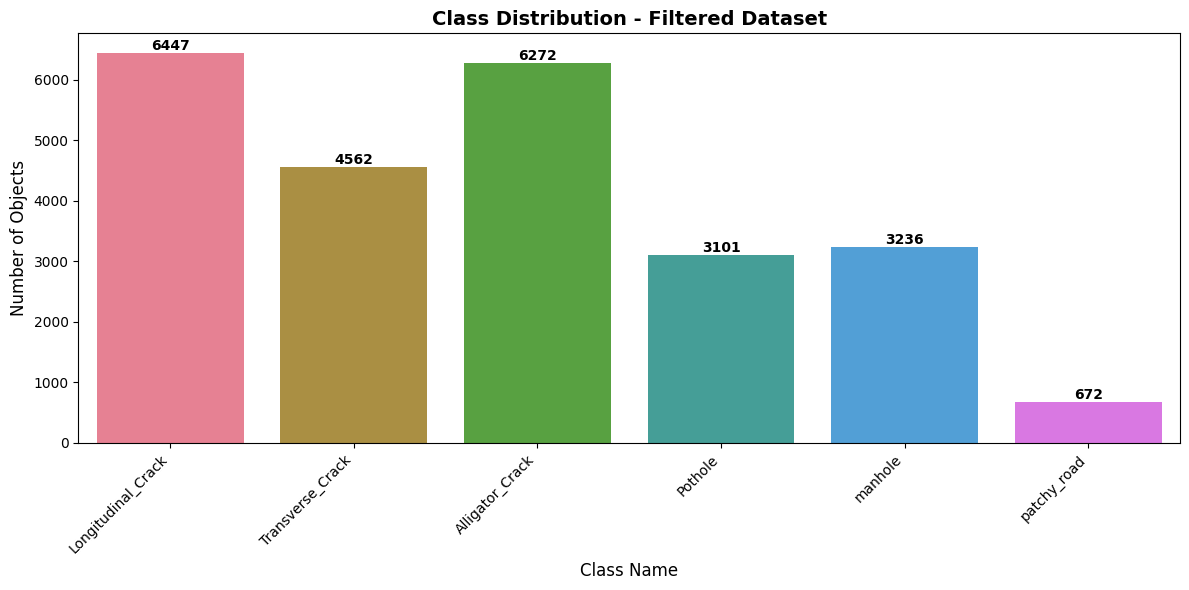
\includegraphics[width=0.85\textwidth]{gambar/distribusi_kelas.png} % Sesuaikan nama file
	\caption{Distribusi Jumlah Objek Berdasarkan Kelas pada Dataset Tersaring}
	\label{fig:distribusi_kelas_global}
\end{figure}

Merujuk pada Gambar \ref{fig:distribusi_kelas_global}, retakan memanjang dan retakan buaya secara berurutan mencatatkan jumlah terbanyak, yaitu 6.447 dan 6.272 objek. Sebaliknya, kelas jalan bertambal (\textit{patchy road}) sangat langka dengan hanya 672 objek. Kelas lubang jalan (\textit{pothole}) dan penutup saluran (\textit{manhole}) juga berada pada kategori minoritas (masing-masing 3.101 dan 3.236 objek). Ketimpangan ini semakin terlihat kompleks ketika dibedah berdasarkan sebaran tiap negara, seperti yang disajikan pada Gambar \ref{fig:distribusi_objek_negara}.

% ==========================================
% GAMBAR: DISTRIBUSI KELAS PER NEGARA
% ==========================================
\begin{figure}[H]
	\centering
	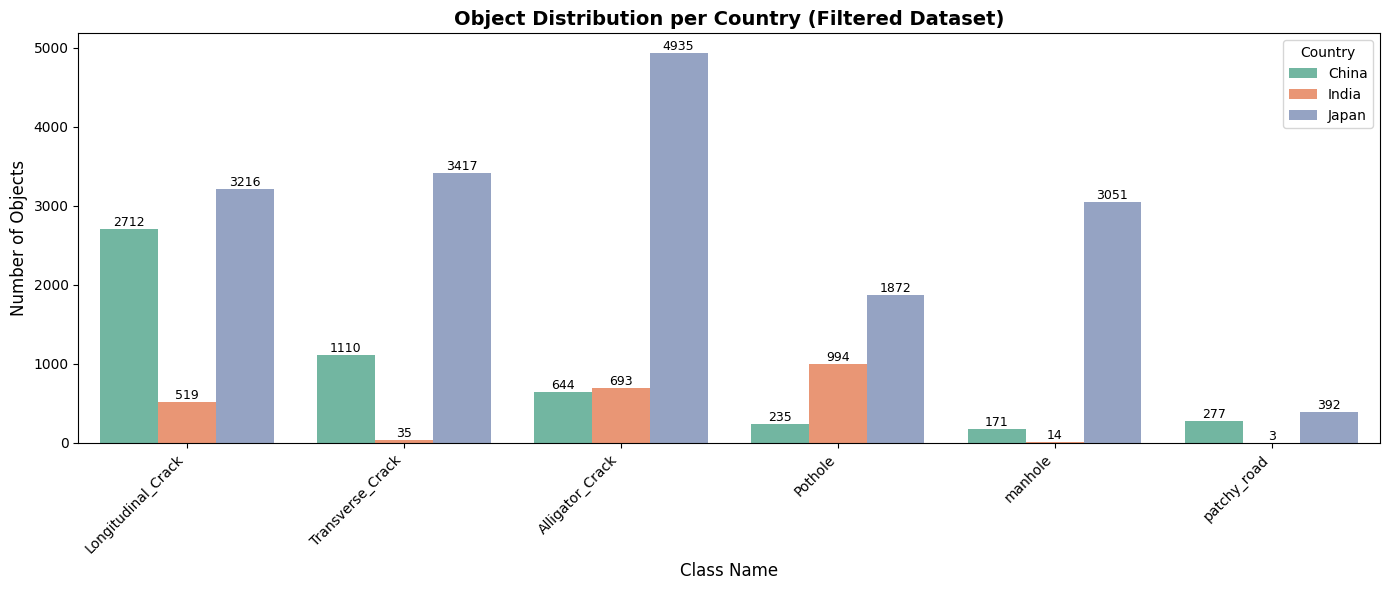
\includegraphics[width=0.9\textwidth]{gambar/distribusi_kelas_country.png} % Sesuaikan nama file
	\caption{Sebaran Jumlah Objek Spesifik per Kelas di Masing-masing Negara}
	\label{fig:distribusi_objek_negara}
\end{figure}

Data dari Gambar \ref{fig:distribusi_objek_negara} menyoroti anomali distribusi lokal. Sebagai contoh, sebagian besar objek \textit{manhole} (3.051 dari 3.236 objek) secara eksklusif bersumber dari Jepang, sementara objek lubang jalan (\textit{pothole}) memiliki proporsi kemunculan yang cukup tinggi di India (994 objek dari total 1.055 citra India) dibandingkan negara lainnya. Fakta empiris terkait ketimpangan kelas yang ekstrem ini menjustifikasi perlunya penerapan modifikasi struktural dan fungsi kerugian adaptif, seperti \textit{Focal Loss}, guna mencegah model bias terhadap kelas mayoritas (retakan) dan mengabaikan objek minoritas (lubang dan pengecoh).

Analisis komprehensif terhadap 24.290 kotak pembatas (\textit{bounding box}) pada dataset tersaring dilakukan untuk melihat proporsi luas objek relatif terhadap luas total citra. Hasil dari analisis metrik tersebut divisualisasikan melalui histogram pada Gambar \ref{fig:distribusi_luas_bbox}.

% ==========================================
% GAMBAR: DISTRIBUSI LUAS BBOX
% ==========================================
\begin{figure}[H]
	\centering
	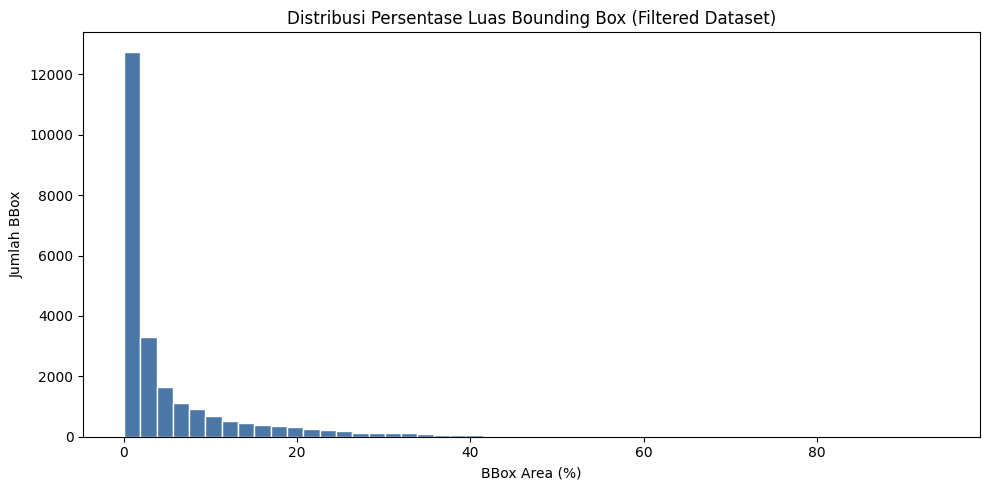
\includegraphics[width=0.9\textwidth]{gambar/distribusi_luas.png} % Sesuaikan nama file
	\caption{Distribusi Persentase Luas \textit{Bounding Box} Terhadap Luas Citra}
	\label{fig:distribusi_luas_bbox}
\end{figure}

Berdasarkan Gambar \ref{fig:distribusi_luas_bbox}, distribusi persentase luas \textit{bounding box} menunjukkan kecondongan positif yang sangat ekstrem (\textit{highly right-skewed}). Nilai median tercatat pada angka 1,69\%, yang mengindikasikan bahwa separuh dari total keseluruhan objek target pada dataset berukuran kurang dari 1,7\% dari total keseluruhan area piksel gambar. Lebih lanjut, metrik persentil ke-90 (P90) yang hanya menyentuh angka 17,19\% menegaskan bahwa keberadaan objek kerusakan berukuran besar sangat jarang ditemukan di lapangan.

Banyaknya objek berukuran sangat kecil dalam dataset ini menjadi tantangan visual tersendiri. Ukuran target yang minim, ditambah dengan tekstur latar belakang jalan raya yang kompleks, membuat anomali tersebut secara alami lebih sulit untuk dikenali secara akurat dalam proses deteksi.

\section{Alur Penelitian}
Penelitian ini dilaksanakan berdasarkan alur penelitian yang dirancang secara terstruktur dan sistematis. Rangkaian tahapan dari proses akuisisi data hingga penarikan kesimpulan divisualisasikan pada diagram alir (\textit{flowchart}) di Gambar \ref{fig:alur_penelitian}.

% ==========================================
% TEMPAT GAMBAR FLOWCHART
% ==========================================
\begin{figure}[H]
	\centering
	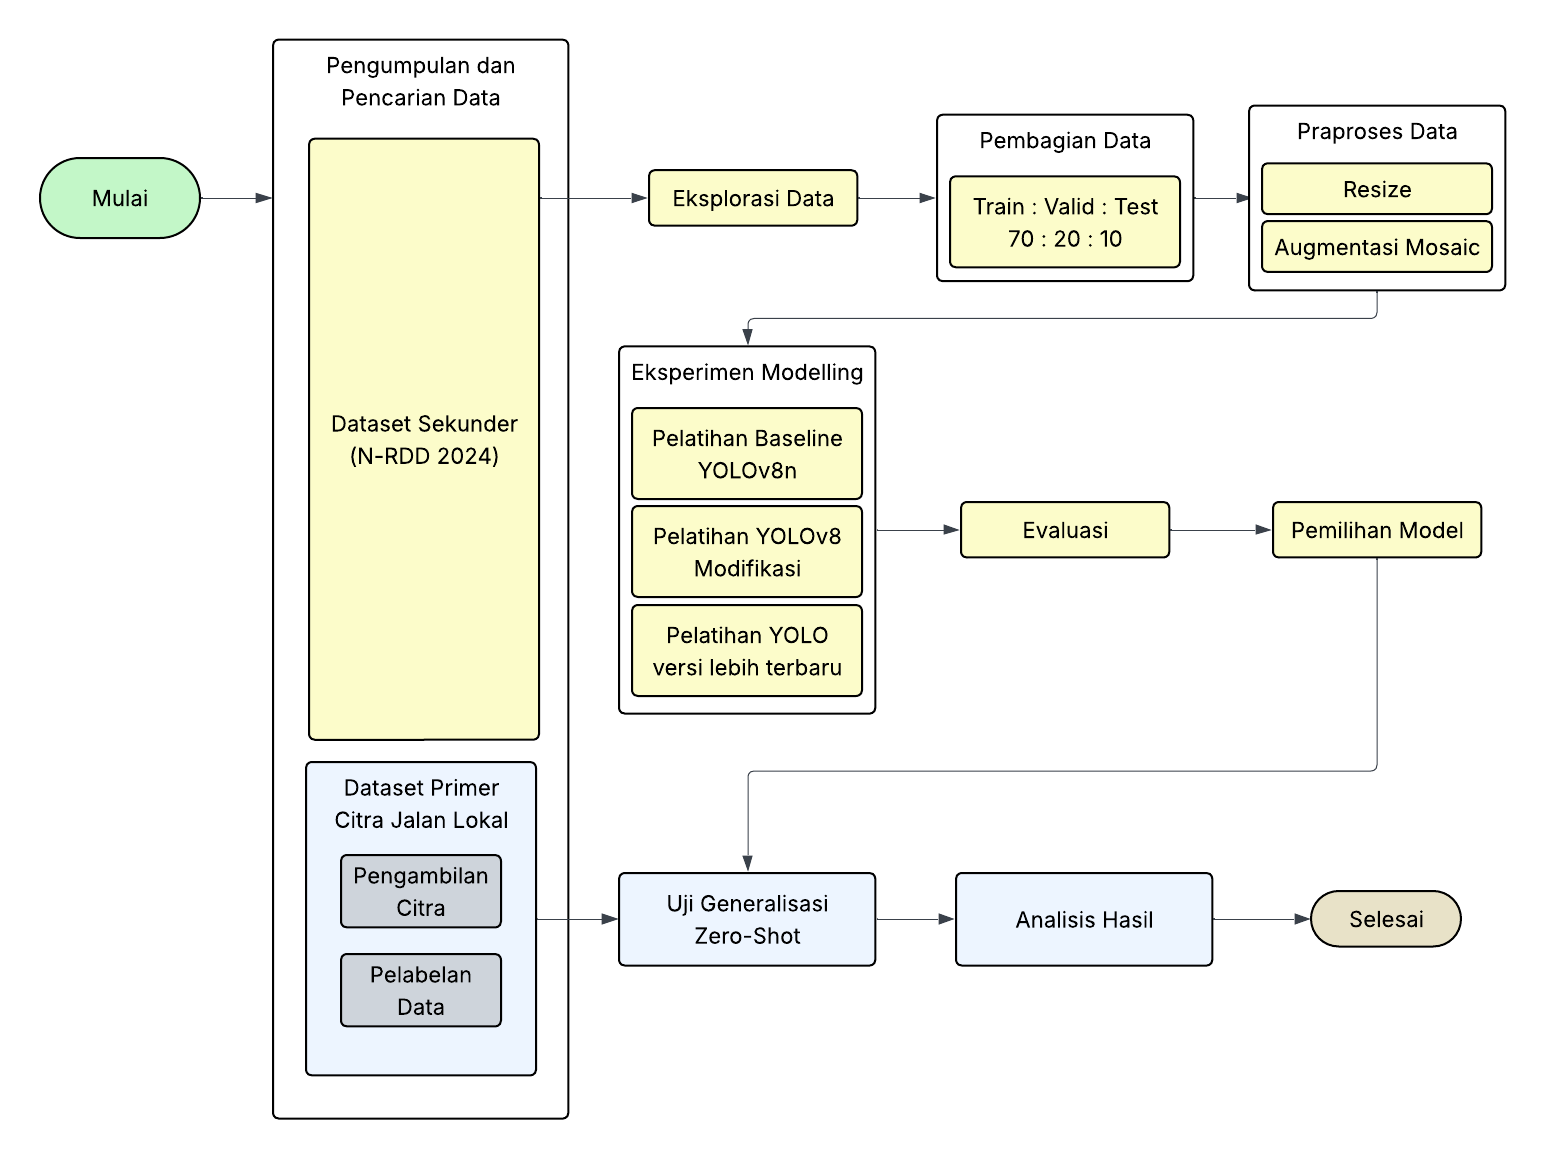
\includegraphics[width=1\textwidth]{gambar/flowchart_penelitian.png}
	\caption{Flowchart Alur Penelitian}
	\label{fig:alur_penelitian}
\end{figure}

Penelitian dimulai dengan pengumpulan data yang terbagi menjadi dua domain utama. Pertama, akuisisi data sekunder menggunakan dataset global \textcolor{blue}{\href{https://data.mendeley.com/datasets/27c8pwsd6v/3}{N-RDD2024}} yang memiliki label kelas kerusakan dan kelas pengecoh secara komprehensif \cite{kaya2024nrdd2024}. Kedua, akuisisi data primer berupa citra jalan raya lokal di  Bandung yang diambil secara mandiri. Karena data primer yang terkumpul masih bersifat mentah, maka dilakukan proses pelabelan secara manual dengan memberikan kotak pembatas (\textit{bounding box}) menggunakan format anotasi standar YOLO agar sesuai dengan kebutuhan inferensi model nantinya.

Setelah data terkumpul, tahap selanjutnya adalah Eksplorasi Data (\textit{Exploratory Data Analysis} / EDA) untuk menganalisis distribusi kelas, ketimpangan data, serta variasi ukuran anomali permukaan jalan. Pemahaman terhadap karakteristik data ini menjadi landasan untuk membagi dataset sekunder (\textit{data splitting}) menjadi himpunan data latih (\textit{train}), data validasi (\textit{validation}), dan data uji (\textit{test}) dengan proporsi 70:20:10.

Himpunan data tersebut kemudian melalui tahap pra-pemrosesan (\textit{preprocessing}). Tahap ini difokuskan pada penyesuaian resolusi citra (\textit{resizing}) menjadi $640 \times 640$ piksel agar sesuai dengan standar ukuran arsitektur masukan (\textit{input size}) keluarga algoritma YOLO \cite{Zeng2024}. Selanjutnya, dilakukan normalisasi nilai piksel serta penerapan teknik augmentasi data seperti \textit{Mosaic}. Augmentasi \textit{Mosaic} bekerja dengan cara menggabungkan empat citra berbeda menjadi satu masukan tunggal, yang secara efektif memperkaya variasi fitur spasial dan melatih model untuk lebih kebal terhadap latar belakang yang kompleks serta variasi skala objek \cite{Zeng2024}.

Tahap pemodelan merancang tiga skenario eksperimen komparatif. Skenario pertama adalah pelatihan model \textit{baseline} menggunakan varian YOLOv8n. Skenario kedua merupakan pelatihan menggunakan arsitektur YOLO yang dimodifikasi (mengikuti penyesuaian arsitektur dari literatur referensi yang relevan dengan dataset). Skenario ketiga menggunakan iterasi algoritma YOLO versi yang lebih baru (seperti YOLOv12 \cite{tian2026yolov12} dan YOLOv26 \cite{sapkota2025yolo26}). Skenario ketiga ini sangat krusial untuk mengevaluasi dan membandingkan apakah peningkatan arsitektur bawaan (\textit{native}) dari versi mutakhir mampu memberikan performa yang lebih tangguh dibandingkan dengan rancangan modifikasi struktural pada iterasi YOLO \textit{baseline}.

Ketiga skenario model tersebut kemudian dievaluasi menggunakan metrik performa deteksi dan metrik efisiensi komputasi untuk menentukan arsitektur dengan keseimbangan kinerja terbaik. Sebagai puncak dari pengujian, model terbaik yang diperoleh dari pelatihan data sekunder akan langsung diuji kemampuannya dalam melakukan generalisasi (\textit{zero-shot inference}) menggunakan dataset primer jalan raya lokal. Uji inferensi ini dilakukan tanpa melatih ulang (\textit{fine-tuning}) model pada data primer, guna mengukur secara objektif ketangguhan arsitektur dalam menghadapi fenomena \textit{domain shift}. Penelitian diakhiri dengan analisis hasil komprehensif atas inferensi \textit{zero-shot} dan penarikan kesimpulan.


\section{Rancangan Arsitektur Model}
Algoritma deteksi objek berbasis keluarga YOLO beroperasi sebagai detektor satu tahap (\textit{one-stage detector}) yang memproses citra secara serentak (\textit{end-to-end}). Pada tahap awal, citra masukan dibagi ke dalam kisi spasial (\textit{grid}) berukuran $S \times S$. Setiap sel pada kisi tersebut secara independen bertanggung jawab untuk memprediksi kotak pembatas (\textit{bounding box}) beserta probabilitas kelas dari objek yang pusat lokasinya jatuh di dalam area sel tersebut \cite{Li2024, Wang2025}. Alur kerja dan topologi dasar dari rancangan arsitektur ini divisualisasikan pada Gambar \ref{fig:arsitektur_yolo}.

% ==========================================
% GAMBAR: ILUSTRASI ARSITEKTUR YOLO
% ==========================================
\begin{figure}[H]
	\centering
	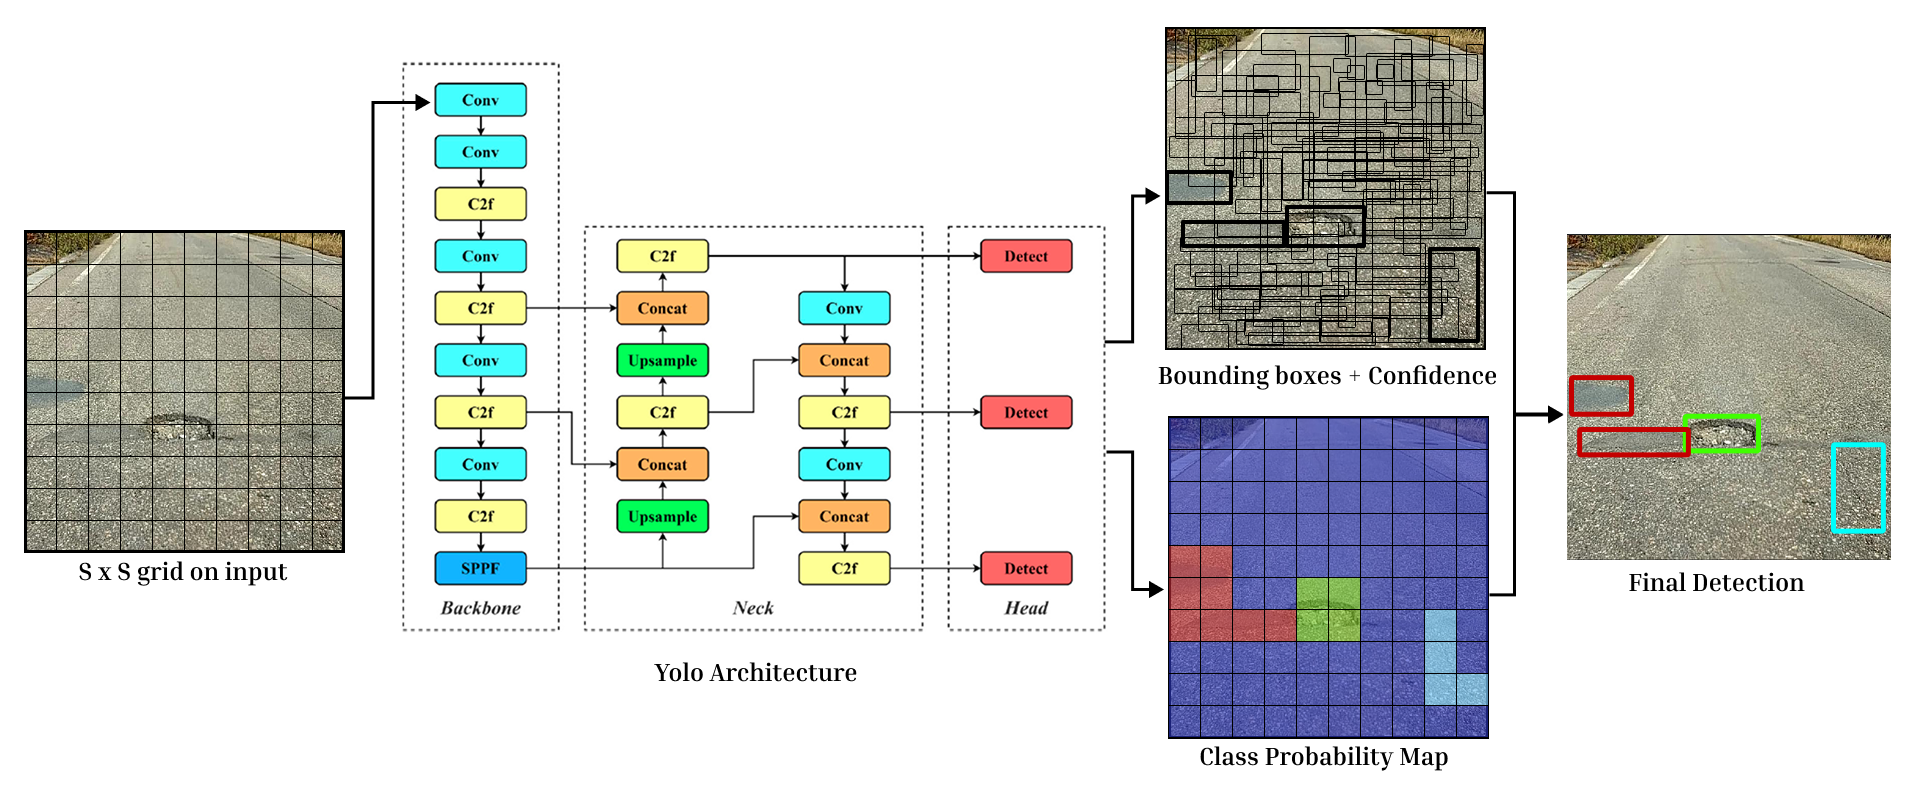
\includegraphics[width=0.9\textwidth]{gambar/rancangan_implementasi.png}
	\caption{Ilustrasi Alur Kerja dan Arsitektur Dasar Jaringan YOLO}
	\label{fig:arsitektur_yolo}
\end{figure}

Secara struktural, rancangan implementasi model jaringan YOLO pada penelitian ini bertumpu pada tiga komponen arsitektur utama, yaitu:
\begin{enumerate}
	\item \textbf{\textit{Backbone}:} Berfungsi sebagai pengekstraksi fitur utama dari citra masukan. Pada iterasi arsitektur mutakhir seperti YOLOv8, komponen ini memanfaatkan kombinasi modul konvolusi standar (Conv), modul C2f (\textit{Cross Stage Partial Bottleneck with 2 convolutions}) untuk memastikan aliran gradien yang kaya dan efisien selama propagasi balik, serta \textit{Spatial Pyramid Pooling - Fast} (SPPF) untuk mengekstrak fitur pada berbagai skala abstraksi spasial \cite{Li2024, Zeng2024}. Untuk meningkatkan sensitivitas terhadap objek berukuran kecil (seperti retakan halus), komponen \textit{backbone} ini sering kali menjadi target utama penyisipan mekanisme atensi, seperti modul SimAM \cite{Li2024} maupun SOM \cite{Wang2025}.

	\item \textbf{\textit{Neck}:} Bertugas melakukan fusi fitur multi-skala. Melalui hierarki operasi \textit{Upsample} dan penggabungan (\textit{Concatenation}), bagian ini memadukan peta fitur beresolusi tinggi (yang kaya akan detail spasial) dengan peta fitur beresolusi rendah (yang kaya akan informasi semantik global) \cite{Li2024, Shi_2026}. Fusi ini memungkinkan model untuk secara adaptif mengenali objek kerusakan jalan dalam rentang skala yang bervariasi. Pada implementasi model modifikasi (\textit{lightweight}), modul konvolusi standar pada \textit{Neck} umumnya digantikan oleh operasi linear hemat biaya seperti \textit{Ghost Convolution} guna mereduksi beban komputasi (GFLOPs) dan menekan redundansi parameter secara drastis \cite{Li2024, Zeng2024, Shi_2026}.

	\item \textbf{\textit{Head}:} Merupakan komponen akhir jaringan yang mengadopsi struktur \textit{decoupled head} untuk memisahkan tugas klasifikasi dan pelokalisasian secara independen. Bagian ini memproses fitur hasil fusi dari \textit{Neck} guna menghasilkan keluaran prediksi secara paralel, yaitu koordinat kotak pelingkup (\textit{bounding boxes}), tingkat metrik keyakinan (\textit{confidence score}), dan probabilitas kelas (\textit{class probability map}) \cite{Li2024, Shi_2026}. Prediksi mentah yang saling tumpang tindih kemudian disaring melalui algoritma \textit{Non-Maximum Suppression} (NMS) untuk menghasilkan keputusan deteksi akhir yang tunggal dan presisi.
\end{enumerate}

\section{Evaluasi Performa Model}
Evaluasi kinerja model pada penelitian ini dibagi menjadi dua aspek utama, yaitu evaluasi ketepatan deteksi (akurasi) dan evaluasi efisiensi komputasi model. Metrik-metrik ini krusial untuk mengukur keberhasilan model, terutama ketika diimplementasikan pada skenario \textit{real-time} dan perangkat dengan sumber daya terbatas \cite{Wu2023}.

\subsection{\textit{Confusion Matrix} (TP, FP, FN)}
Dalam tugas deteksi objek, landasan utama perhitungan metrik evaluasi bersumber dari \textit{Confusion Matrix} yang didefinisikan berdasarkan ambang batas \textit{Intersection over Union} (IoU). Matriks ini mengelompokkan hasil prediksi ke dalam tiga kondisi \cite{Li2024, Zeng2024}:
\begin{itemize}
	\item \textbf{\textit{True Positive} (TP):} Model berhasil memprediksi objek kerusakan jalan dengan benar, kelasnya sesuai dengan \textit{ground truth}, dan nilai IoU melampaui ambang batas yang ditentukan (misalnya IoU $>$ 0,5).
	\item \textbf{\textit{False Positive} (FP):} Model mendeteksi adanya objek kerusakan jalan di lokasi tertentu, padahal pada kondisi asli (\textit{ground truth}) tidak terdapat kerusakan (salah deteksi) atau kelas yang diprediksi keliru.
	\item \textbf{\textit{False Negative} (FN):} Terdapat kerusakan jalan pada kondisi nyata, namun model gagal mendeteksi atau melokalisasi kerusakan tersebut (\textit{missed detection}).
\end{itemize}

\subsection{\textit{Precision, Recall}, dan F1-\textit{Score}}
Berdasarkan nilai TP, FP, dan FN, kinerja klasifikasi model dapat diukur menggunakan tiga metrik turunan. \textit{Precision} mengukur tingkat ketepatan prediksi positif dari model, sedangkan \textit{Recall} (sensitivitas) mengukur kemampuan model dalam menemukan seluruh objek kerusakan yang sebenarnya ada di dalam citra \cite{Zeng2024, Li2024}.
\begin{equation}
	Precision = \frac{TP}{TP + FP}
\end{equation}
\begin{equation}
	Recall = \frac{TP}{TP + FN}
\end{equation}
Karena \textit{Precision} dan \textit{Recall} sering kali berbanding terbalik, digunakan metrik F1-\textit{Score} yang merupakan rata-rata harmonis dari keduanya. Metrik ini memberikan penilaian yang seimbang dan komprehensif terkait ketangguhan model \cite{Li2024}.
\begin{equation}
	F1\text{-}Score = 2 \times \frac{Precision \times Recall}{Precision + Recall}
\end{equation}

\subsection{\textit{Intersection over Union} (IoU) dan \textit{Mean Average Precision} (mAP)}
\textit{Intersection over Union} (IoU) mengukur seberapa akurat lokalisasi kotak pembatas (\textit{bounding box}) yang diprediksi oleh model dibandingkan dengan kotak pembatas asli (\textit{ground truth}) \cite{Li2024}.
\begin{equation}
	IoU = \frac{Area \ of \ Overlap}{Area \ of \ Union}
\end{equation}
Dari perhitungan presisi pada berbagai ambang batas \textit{Recall}, diperoleh nilai \textit{Average Precision} (AP). Rata-rata AP dari seluruh kelas objek kemudian dirumuskan menjadi \textit{Mean Average Precision} (mAP), yang merupakan metrik standar tertinggi dalam deteksi objek \cite{Wu2023, Li2024}:
\begin{equation}
	mAP = \frac{1}{N} \sum_{i=1}^{N} AP_i
\end{equation}
Dalam penelitian ini, selain menggunakan metrik mAP@0.5 (mAP pada IoU 50\%), digunakan pula metrik evaluasi multi-skala seperti mAP$_s$ (untuk objek berukuran sangat kecil $< 32\times32$ piksel), mAP$_m$ (skala menengah), dan mAP$_l$ (skala besar) untuk menganalisis sensitivitas model terhadap variasi ukuran retakan jalan yang ekstrem \cite{Wang2025}.

\subsection{Metrik Efisiensi Komputasi}
Untuk mengukur kelayakan model pada perangkat komputasi bergerak (\textit{mobile terminal devices}), digunakan tiga metrik evaluasi efisiensi \cite{Wu2023, Wang2025}:
\begin{itemize}
	\item \textbf{\textit{Parameters} (Params):} Total kuantitas bobot yang dapat dipelajari (\textit{learnable parameters}) dalam jaringan saraf. Metrik ini, biasanya dalam satuan \textit{Million} (M), mengukur kompleksitas spasial dan ukuran ruang penyimpanan model.
	\item \textbf{GFLOPs (\textit{Giga Floating-Point Operations Per Second}):} Kuantitas operasi komputasi yang dibutuhkan model dalam satu kali inferensi. Metrik ini secara langsung merepresentasikan beban komputasi jaringan.
	\item \textbf{FPS (\textit{Frames Per Second}):} Indikator langsung dari kecepatan inferensi model dalam memproses citra per detiknya, yang menentukan kelayakan sistem untuk skenario pengawasan \textit{real-time}.
\end{itemize}

\section{Skenario Penelitian}
Skenario pengujian merupakan inti eksperimental dari metodologi penelitian ini. Untuk menjawab ketiga rumusan masalah yang telah ditetapkan pada Bab 1 secara sistematis, skenario penelitian ini dipecah ke dalam tiga tahapan evaluasi utama:

\subsection{Skenario 1: Evaluasi Kinerja pada Domain Sumber dan Analisis Kelas Pengecoh}
Skenario pertama dirancang secara komparatif untuk melatih dan mengevaluasi konfigurasi arsitektur model menggunakan dataset sekunder N-RDD2024. Penelitian ini menguji YOLOv8n sebagai model \textit{baseline}, rancangan eksperimental model modifikasi yang dikonfigurasi dengan mengeksplorasi berbagai modul optimasi (seperti mekanisme atensi dan konvolusi ringan) yang diadaptasi dari arsitektur mutakhir seperti YOLO-RD \cite{Wang2025}, RDD-YOLO \cite{Li2024}, maupun YOLOv8-PD \cite{Zeng2024}, serta iterasi algoritma versi mutakhir berupa YOLOv12 \cite{tian2026yolov12} dan YOLOv26 \cite{sapkota2025yolo26}. Fokus utama pada tahap ini adalah mengukur tingkat akurasi (mAP) dari masing-masing arsitektur dalam mendeteksi kelas kerusakan jalan utama. Bersamaan dengan itu, evaluasi juga diarahkan untuk mengamati bagaimana model menangani ketimpangan data (\textit{class imbalance}) serta kemampuannya dalam membedakan kerusakan jalan asli dari kelas pengecoh berupa penutup saluran air (D70) dan tambalan aspal (D80). Kemampuan arsitektur dalam menghindari kebingungan visual terhadap objek pengecoh ini dibuktikan secara empiris melalui analisis maatriks kebingungan (\textit{Confusion Matrix}) guna melihat tingkat penekanan \textit{false positive}. Untuk memastikan model tidak bias terhadap kelas mayoritas selama proses pelatihan, strategi penanganan ketimpangan kelas melalui penerapan fungsi kerugian adaptif (\textit{Focal Loss}) atau pembobotan kelas bawaan dari kerangka kerja YOLO. Skenario ini akan menghasilkan capaian metrik mAP dan F1-\textit{Score} murni pada domain sumber yang menjadi \textit{benchmark} performa standar model.


\subsection{Skenario 2: Analisis Keseimbangan Kinerja (\textit{Trade-Off}) dan Kelayakan \textit{Real-Time}}
Skenario kedua berfokus pada analisis kelayakan penerapan model pada skenario \textit{real-time} dengan sumber daya komputasi terbatas. Pada tahap ini, metrik akurasi (mAP) dari model-model yang telah dilatih pada Skenario 1 akan dibandingkan dengan metrik efisiensi komputasinya, yang meliputi kecepatan inferensi (FPS), jumlah parameter (\textit{Params}), dan beban operasi (\textit{GFLOPs}). Seluruh pengujian efisiensi komputasi ini akan dievaluasi menggunakan perangkat keras NVIDIA RTX 4070 Ti 12GB sebagai basis tolok ukur (benchmark).Analisis keseimbangan kinerja (\textit{trade-off}) ini akan menentukan apakah modifikasi arsitektur \textit{lightweight} benar-benar mampu memberikan titik optimal terbaik antara menekan beban komputasi secara signifikan tanpa mengorbankan ketepatan deteksi. Dari skenario evaluasi komputasi ini, akan dipilih satu model terbaik untuk dilanjutkan ke tahap evaluasi akhir.

\subsection{Skenario 3: Uji Ketangguhan Lintas Domain (\textit{Zero-Shot Inference})}
Skenario ketiga bertujuan untuk mengukur secara kuantitatif tingkat kesenjangan domain (\textit{domain gap}) dari model terbaik yang telah terpilih. Model terbaik dari hasil analisis komputasi Skenario 2 akan diekstraksi bobotnya (\textit{weights}) dan diuji secara langsung (\textit{zero-shot}) menggunakan dataset primer jalan raya Bandung, tanpa memberikan model kesempatan untuk melakukan \textit{fine-tuning}. tahap evaluasi akhir ini akan membuktikan kemampuan generalisasi murni model dalam menghadapi data baru (\textit{unseen data}). Perbedaan selisih akurasi (\textit{accuracy drop}) antara kinerja di Skenario 1 dan Skenario 3 akan dianalisis sebagai representasi besaran \textit{domain shift}.
